\documentclass[10pt,slovak,a4paper]{article}

\usepackage[slovak]{babel}
\usepackage[IL2]{fontenc} 
\usepackage[utf8]{inputenc}
\usepackage{graphicx}
\usepackage{url}
\usepackage{hyperref}
\usepackage{cite}
\usepackage{amsmath}

\pagestyle{headings}

\title{Algoritmy odporúčania filmov v Netflix\thanks{Semestrálny projekt v predmete Metódy inžinierskej práce, ak. rok 2024/25, vedenie: Ing. Richard Marko, PhD}}

\author{Yehor Bohuslavskyi\\[2pt]
	{\small Slovenská technická univerzita v Bratislave}\\
	{\small Fakulta informatiky a informačných technológií}\\
	{\small \texttt{xbohuslavkyi@stuba.sk}}
	}

\date{\small 17. oktober 2024}

\begin{document}

\begin{figure}[h!]
  \centering
  
\includegraphics[width=\textwidth]{Images/fiit_logo.png} 
\end{figure}

\maketitle

\begin{abstract}
Túto tému som si vybral, pretože je veľmi zaujímavé, ako technológie a umelá inteligencia(ktorá je v súčasnosti jednou z najrozvíjajúcejších sa tém) ovplyvňujú naše každodenné rozhodovanie o tom, čo sledujeme. Ja som zvedavý, že ako po zhliadnutí jedného tureckého filmu, ktorý som ani neohodnotil, sa mi v odporúčaniach začali objavovať podobné filmy. 

V systéme sa nachádza viac, ako 15 000 filmov a zobrazuje vám len tie, ktoré sa vám budú páčiť (neskôr dozvieme sa, ako to funguje). Fakt: ani jeden používateľ Netflix nebol by schopný si samostatne nájsť film alebo seriál, ktorý by sa mu páčil bez požívania algoritmu odporúčania filmov \cite{Netflix:Algorithm}.
 
V tomto článku sa podrobne pozrieme na algoritmy spoločnosti Netflix. V súčasnosti je systém Netflix postavený na algoritme, ktorý využíva umelú inteligenciu a strojové učenie. Pozrieme sa aj na umiestnenie odporúčaní na obrazovke, kde je niekoľko typov návrhov. Prvým je „Odporúčané pre vás“, po ňom idú „Trendy“, na stránke sa nachádza aj záložka „New Releases“\cite{Netflix:Recommendation:System}.

Podrobne sa pozrieme aj na filtračné algoritmy, ktoré sa delia na dva hlavné typy. Akú rolu odohrávajú hodnotenia a správania používateľov v rámci algoritmu collaborative filtering a „filtrovanie na základe obsahu“.

Zaujímavým aspektom sú aj systémy hodnotenia. Patrí medzi ne „Personalizované hodnotenie videa (PVR)“, „Top-N Ranking“, „Rebríček obľúbených filmov“ a „Zoznam zaujímavého obsahu na neskoršie sledovanie“. Každé z týchto hodnotení je personalizované pre jednotlivých používateľov, čo je veľmi zaujímavé.

V rámci článku sa budeme venovať aj typom údajov, ktoré Netflix používa. Tie sa zhruba delia na dva typy: základné typy zhromažďovaných údajov a dodatočné informácie. Medzi základné patria „interakcie používateľa so stránkou“, ktoré pozostávajú z histórie sledovania a hodnotení. Druhým typom sú „korelačné údaje“, „informácie o obsahu knižnice Netflix“, ako napríklad žánre. Ďalšie uvidíme ako ovplyvňujú  špecifickejšie typy informácií, ako sú napríklad denný čas, používané zariadenie alebo priemerná dĺžka sledovania.

\end{abstract}

\section{Úvod}
Cieľom spoločnosti Netflix je používať odporúčacie algoritmy na maximalizáciu spokojnosti
používateľov. Hlavným cieľom je prispôsobiť obsah každému jednotlivému používateľovi.

Netflix má obrovskú knižnicu obsahu a obmedzené rozhranie obrazovky, čo veľmi sťažuje odporúčanie relevantného obsahu, a každý používateľ má iný vkus, preferencie a zvyky pri sledovaní, takže personalizácia musí byť veľmi presná.\cite{Bennett}
Čo robí Netflix na dosiahnutie tohto cieľa, sa dozviete po tomto článku.

\section{Technológie a Umelá inteligencia v Netflix}
V súčasnosti veľké spoločnosti v IT priemysle využívajú umelú inteligenciu, čo nezostalo bez povšimnutia spoločnosti Netflix, ktorá kombinuje niekoľko modelov a prístupov (tzv. ensemble learning) na vytvorenie najlepších odporúčaní.\cite{Bennett}

\section{Typy Odporúčaní na Netflix}
Netflix používa dvoj úrovňový systém hodnotenia založený na riadkoch, čo to znamená? Obsah je hodnotený dvakrát, v stĺpcoch a v každom riadku, ako sa dozviete v článku ďalej.
Na základe kombinácie týchto prístupov sa vytvárajú personalizované odporúčania pre konkrétneho používateľa.\cite{Habr}

\begin{figure}[h!]
  \centering
  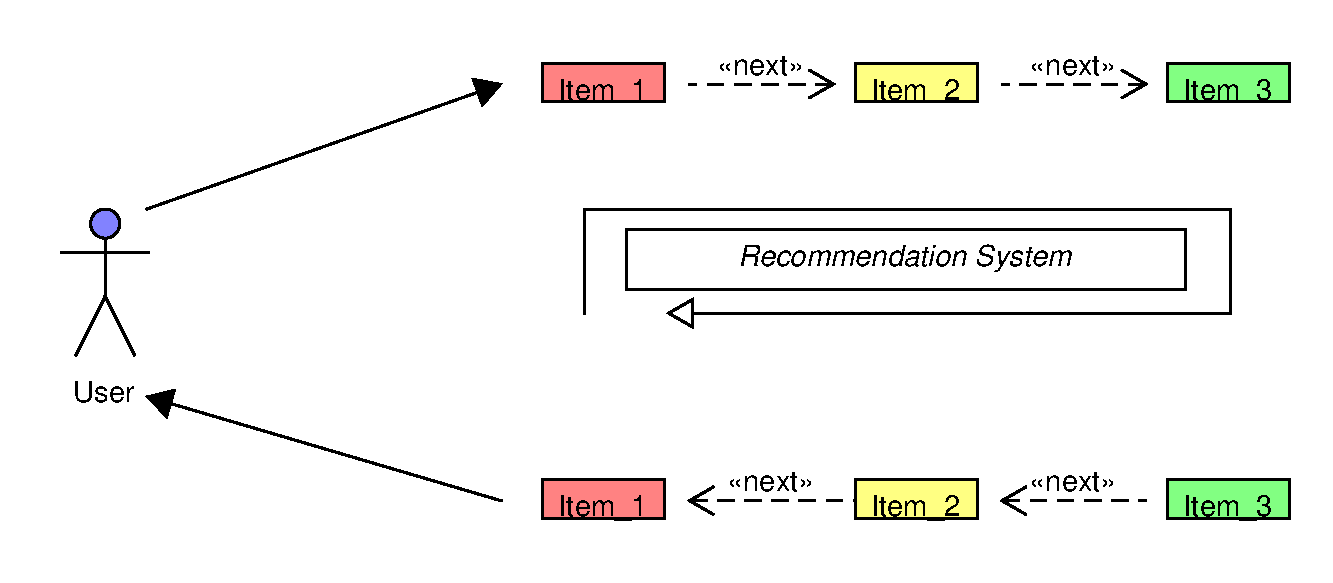
\includegraphics[width=1\textwidth]{Images/RecommendationSystem_pdf.pdf} % Adjust width as needed
  \caption{Recommendation System}
\end{figure}

\section{Filtračné algoritmy}
Porovnanie a vysvetlenie algoritmov collaborative filtering a filtrovania na základe obsahu.
Vplyv hodnotení a správania používateľov na úspešnosť algoritmov.

\begin{figure}[h!]
  \centering
  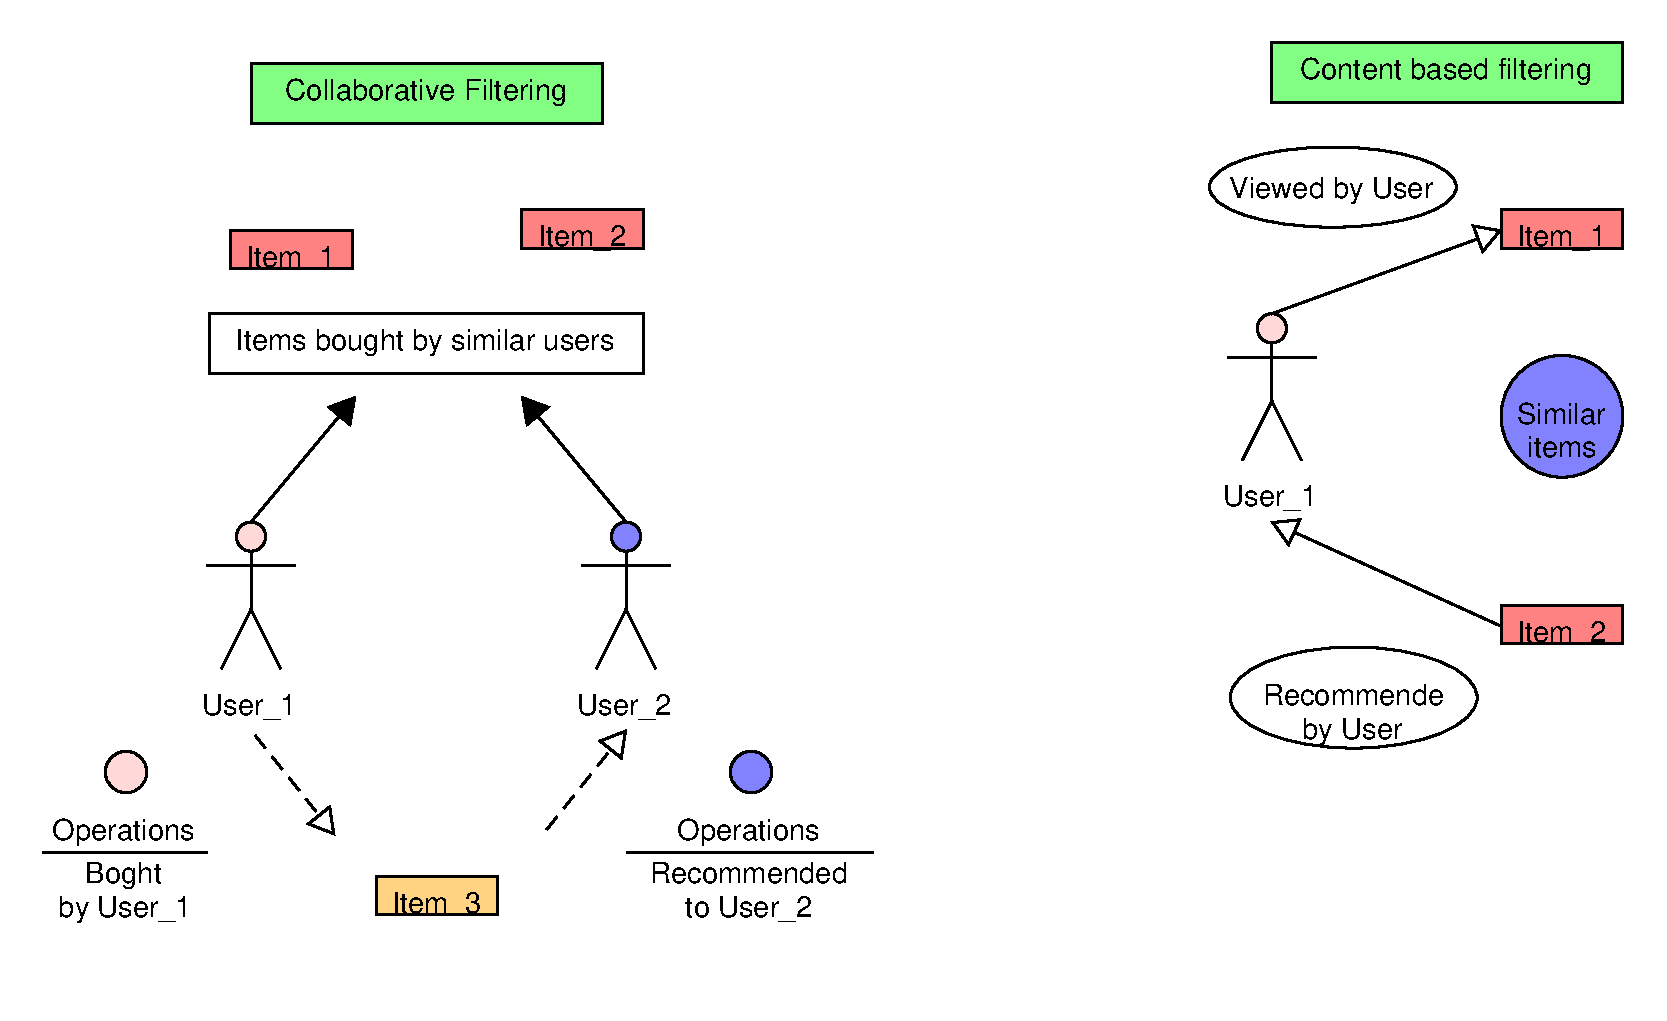
\includegraphics[width=1\textwidth]{Images/Filtering_pdf.pdf} % Adjust width as needed
  \caption{Type of Filtering}
\end{figure}

\section{Systémy Hodnotenia}
Prehľad o rôznych systémoch hodnotenia (Personalizované hodnotenie videa, Top-N Ranking, Rebríčky obľúbených filmov, Zoznam zaujímavého obsahu na neskoršie sledovanie).
Ako tieto systémy prispievajú k osobnej skúsenosti používateľov.

\section{Typy Údajov v Netflix}
Spoločnosť Netflix tiež zhromažďuje množstvo údajov o svojich používateľoch, ktoré používa na optimalizáciu odporúčaní. Možno vás zaujíma, čo sú to za údaje a ako ich najväčšia online platforma využíva, aj to sa dozviete v tomto článku.\cite{Bennett}

\section{Vplyv špecifickejších informácií}
Analýza vplyvu denného času, používaného zariadenia a priemerného času sledovania na odporúčacie algoritmy Netflixu.

\section{Záver}
Odporúčací systém Netflixu je zložitý mechanizmus, ktorý využíva sofistikované algoritmy na spracovanie veľkého množstva údajov a preferencií používateľov. Je to kľúčový nástroj na udržanie záujmu používateľov a na to, aby sa nestratili v obrovskej knižnici obsahu.

\bibliography{literatura}
\bibliographystyle{plain}

\end{document}
